\documentclass[preprint,12pt]{elsarticle}

\usepackage{iftex}
\ifXeTeX\else
  \errmessage{This manuscript must be compiled with XeLaTeX.}
\fi
\usepackage{fontspec}
\usepackage{xeCJK}
\IfFontExistsTF{Times New Roman}{\setmainfont{Times New Roman}}{\setmainfont{TeX Gyre Termes}}
\IfFontExistsTF{SimSun}{\setCJKmainfont{SimSun}}{\setCJKmainfont{FandolSong-Regular}}
\IfFontExistsTF{Microsoft YaHei}{\setCJKsansfont{Microsoft YaHei}}{\setCJKsansfont{FandolHei-Regular}}
\IfFontExistsTF{FangSong}{\setCJKmonofont{FangSong}}{\setCJKmonofont{FandolFang-Regular}}
\IfFontExistsTF{Consolas}{\setmonofont{Consolas}}{\setmonofont{Courier New}}

\usepackage{amsmath,amssymb}
\usepackage{booktabs}
\usepackage{multirow}
\usepackage{graphicx}
\usepackage{subcaption}
\usepackage{siunitx}
\usepackage{float}
\usepackage{hyperref}
\usepackage{enumitem}
\usepackage{threeparttable}
\usepackage{longtable}
\usepackage{xcolor}

\graphicspath{{../picture/}}
\hypersetup{colorlinks=true,linkcolor=black,citecolor=blue,urlcolor=blue}
\journal{SCI期刊投稿稿（中文整理版）}
\biboptions{numbers,sort&compress}

\title{一种面向无人机目标跟踪控制的显式门控双状态洁净偏差重建方法}

\author[aff1]{作者甲}
\author[aff1]{作者乙}
\author[aff2]{作者丙\corref{cor1}}
\cortext[cor1]{通信作者信息请在正式投稿前替换。}
\address[aff1]{单位一，城市，邮编，中国}
\address[aff2]{单位二，城市，邮编，中国}

\begin{document}
\begin{frontmatter}

\begin{abstract}
针对无人机目标检测后进入跟踪控制链时原始偏差序列抖动大、丢失恢复敏感且直接影响电机输入的问题，本文围绕 current clean offset reconstruction 任务，提出一种显式门控双状态洁净偏差重建方法。该方法以跟踪日志中的原始偏差、滤波状态、检测置信度、丢失标志和测量年龄等字段为输入，采用“传统预滤波基线 + 事件分支残差修正”的结构：低门控区域使用传感器侧指数滑动平均输出作为稳态基线，高门控区域使用短窗滑动平均加残差分支进行事件重建，并通过显式事件门控在高抖动、丢失恢复和快速转折场景中选择更合适的路径。本文构建了真实采集的跟踪后日志数据集，建立了标签校验、门禁筛选、离线训练、ONNX 导出和 C++ 在线接入的完整流程。实验结果表明，在正式验证集上，所提 dual-state 模型的 overall RMSE 为 25.5309\,px，优于 Raw（26.1366\,px）、EMA（25.7461\,px）和 SMA（26.0915\,px）；在 high\_jitter、lost\_coasting 和 fast\_turn 三类关键分段上，RMSE 分别达到 9.4197\,px、39.3532\,px 和 3.6723\,px，均优于上述传统基线。五个随机种子的复验结果表明，该模型的 overall RMSE 落在 25.5164--25.5480\,px 之间，具有良好的重复性。最后，本文将最优模型导出为 ONNX 并接入 C++ 跟踪控制链，在回放与相机 smoke 测试中均验证了在线推理链路的有效性。
\end{abstract}

\begin{keyword}
无人机目标跟踪 \sep 洁净偏差重建 \sep 显式门控 \sep 双状态模型 \sep 传统滤波 \sep 在线部署
\end{keyword}

\end{frontmatter}

\section{引言}
无人机目标跟踪控制链通常包含检测、跟踪、偏差估计和电机控制四个环节。对于下游 PID 控制而言，真正重要的不是图像级别检测本身，而是当前时刻可直接送入控制器的二维偏差量。工程上常用的 Raw、指数滑动平均（EMA）、滑动平均（SMA）、卡尔曼滤波和 IMM 等方法具有实现简单、推理稳定的优点，但在高抖动、丢失恢复和快速转折等事件场景中，往往需要在噪声抑制与响应延迟之间做固定折中；其中卡尔曼滤波与多模型估计是经典基线，SORT、DeepSORT、ByteTrack 与 BoT-SORT 则代表了工程中常见的检测后跟踪路线\cite{kalman1960new,barshalom2001estimation,bewley2016sort,wojke2017deepsort,zhang2022bytetrack,aharon2022botsort}。本文的目标不是取代目标跟踪器本身，而是在“检测后、控制前”的狭义接口上，重建一条更适合作为电机输入的 clean offset。

围绕这一目标，本文将问题限定为 stage1 clean-only 任务：输入为跟踪器已经产生的偏差与状态字段，输出为当前 clean offset。与同时预测 future head 或 delay-aware 目标的多任务框架不同，本文只优化当前时刻的 clean reconstruction，并使用统一分段指标对 stable、jitter、recover 和 turn 四类真实场景进行验证。实验表明，当模型主干没有正确约束时，神经网络很容易退化为“比传统滤波更差的低通器”；因此本文的关键不是盲目加大网络规模，而是把传统滤波、事件门控和残差学习组合到同一条可部署链路中。本文中使用的 TCN 与 GRU 结构选择分别参考了序列建模和门控循环建模中的典型做法\cite{bai2018empirical,cho2014learning}。

本文的主要贡献如下：
\begin{enumerate}[label=\arabic*)]
  \item 提出一种面向控制输入的显式门控双状态 clean-only 结构，在稳态区间使用 EMA 基线，在事件区间使用短窗滑动平均加残差修正，并以显式事件门控控制两条路径的切换。
  \item 构建了一套从真实跟踪日志采集、标签校验、门禁筛选、数据集构建、基线对比到 ONNX 在线接入的完整工程流程，使 clean offset 研究能够在真实控制接口上闭环。
  \item 在正式验证集上，所提 dual-state 模型在 overall、high\_jitter、lost\_coasting 和 fast\_turn 四个关键口径上均优于 Raw、EMA 和 SMA 基线，并通过五个随机种子复验给出稳定性证据。
\end{enumerate}

\section{问题定义与数据流程}
\subsection{控制接口与任务定义}
设原始跟踪偏差为 $\mathbf{u}_t=[dx_t,dy_t]^\top$，其来源于跟踪器对目标框中心与图像中心的偏差估计。控制链所需的 clean offset 记为 $\hat{\mathbf{u}}_t$。本文不预测未来轨迹，也不显式拟合控制时延，而是只学习当前时刻的 clean reconstruction：
\begin{equation}
\hat{\mathbf{u}}_t = f(\mathcal{X}_{t-L+1:t}),
\end{equation}
其中 $L=16$ 为时间窗口长度，$\mathcal{X}_{t-L+1:t}$ 包含原始偏差、差分特征、趋势特征、检测置信度、丢失状态、测量年龄、变焦变化、转折分数和切换分数等 20 维输入。

\subsection{真实日志采集与标签校验}
本文使用的是目标检测后、目标跟踪后的 full log，而非原始图像序列。采集日志经过单段校验和批量汇总后再进入训练。按最新数据报告，原始日志共包含 27\,342 帧、33 个片段；按场景标签统计，stable、recover、jitter、turn 和 zoom 的片段数量分别为 16、7、4、4 和 2。考虑部署策略中目标锁定后不以变焦段为主验证口径，最终 stage1 的门禁类型固定为 stable、jitter、recover 和 turn 四类。经校验后的可用来源数量为 stable=1、jitter=1、recover=2、turn=4。

图 \ref{fig:pipeline} 给出了本文的整体流程：跟踪器产生原始偏差和状态字段后，先经过传统滤波基线构造，再输入显式门控双状态模型，输出 clean offset 供 PID 使用；同时全流程支持 ONNX 导出和 C++ 侧在线调用。

\begin{figure}[H]
  \centering
  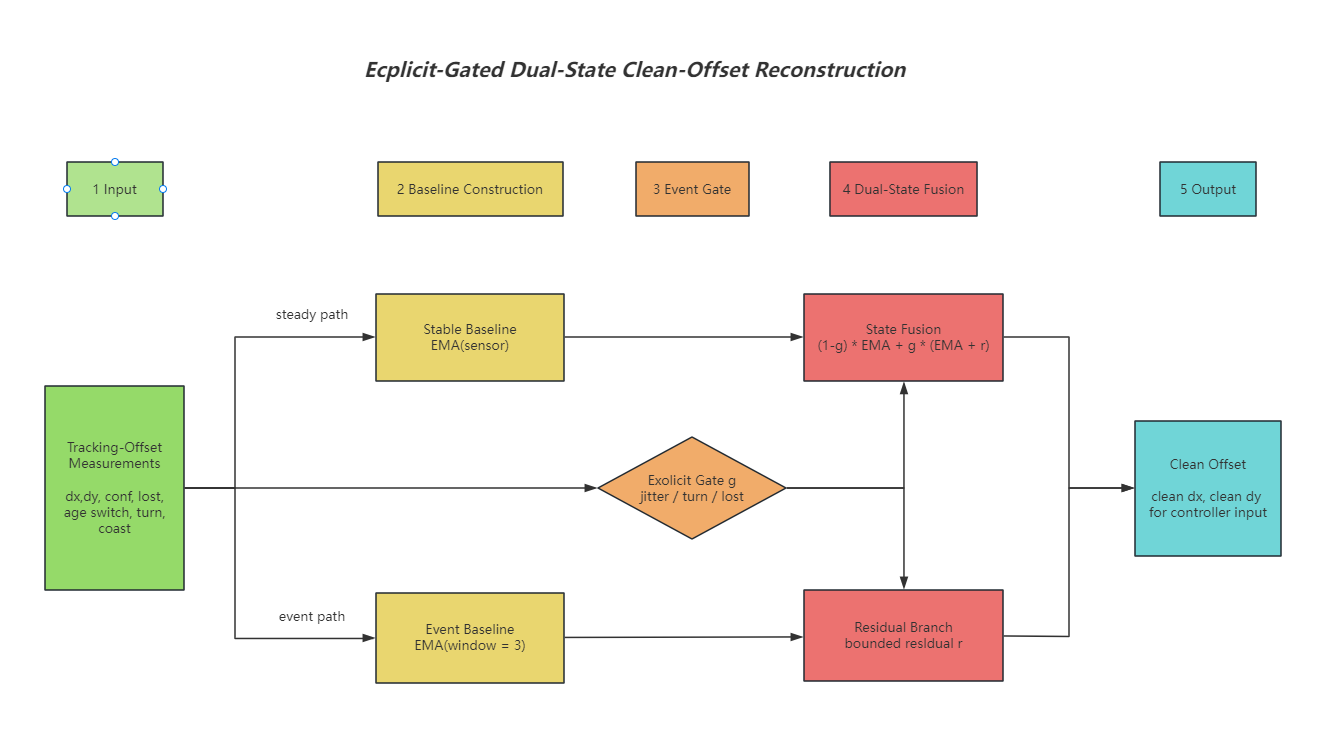
\includegraphics[width=\linewidth]{fig_pipeline.png}
  \caption{Stage1 clean-only 推理流程。}
  \label{fig:pipeline}
\end{figure}

\subsection{数据规模与切分}
数据集构建阶段先按片段切分，再在片段内部切窗，最后按来源组进行 train/val/test 分配，避免同一原始日志的不同子段同时落入训练集与测试集。正式数据报告显示，总样本窗口数为 5\,256，其中训练、验证和测试窗口分别为 3\,927、233 和 1\,096。本文所有模型与基线均在同一测试口径上比较，评价指标包括 MAE、RMSE、switch\_segment\_lag、turn\_point\_retention\_error 和 jitter\_energy。

\section{方法}
\subsection{传统预滤波基线}
直接将神经网络作用在生噪的 tracking offset 上，会使模型倾向于学习一个不稳定的低通器。为此，本文首先构造两条传统滤波基线：
\begin{align}
\mathbf{b}^{\mathrm{ema}}_t &= \mathrm{EMA}(\mathbf{u}_{1:t}),\\
\mathbf{b}^{\mathrm{sma}}_t &= \mathrm{SMA}_3(\mathbf{u}_{t-2:t}),
\end{align}
其中 $\mathbf{b}^{\mathrm{ema}}_t$ 作为稳态基线，$\mathbf{b}^{\mathrm{sma}}_t$ 作为事件区间的短窗基线。模型不再从零开始拟合 clean offset，而是围绕这两条传统基线进行有约束的残差修正；这种设计本质上是在传统状态估计器之外增加一层面向控制接口的补偿器，而不是直接替换经典滤波器\cite{kalman1960new,barshalom2001estimation}。

\subsection{显式门控双状态结构}
为了避免 learned gate 在小数据场景下塌缩为常开，本文最终采用显式事件门控。定义门控值 $g_t\in[0,1]$，其由切换分数、转折分数、丢失标志和海岸计数等事件特征线性组合并裁剪得到。模型输出定义为
\begin{equation}
\hat{\mathbf{u}}_t = (1-g_t)\mathbf{b}^{\mathrm{ema}}_t + g_t\left(\mathbf{b}^{\mathrm{sma}}_t + \mathbf{r}_t\right),
\end{equation}
其中 $\mathbf{r}_t$ 为事件分支残差。这样的结构具有两个直接好处：其一，稳态区间至少不会比 EMA 基线更差；其二，事件区间的学习目标从“直接重建 clean offset”收缩为“在短窗平滑基线上做有限修正”。

\subsection{教师信号与损失设计}
本文的 teacher 不再单纯依赖跟踪器内部的 $dx\_hat/dy\_hat$，而是根据场景分段采用不同的融合策略。在 stable 段，以 $dx\_hat/dy\_hat$ 与因果趋势项为主；在 jitter 段，显著提高 raw、短窗 EMA 和 rolling median 的占比；在 recover 段，强调 last-good 状态与 gradual re-entry；在 turn 段，提高 raw 与短窗 EMA 权重，降低对内部滤波状态的依赖。损失函数由四部分构成：
\begin{equation}
\mathcal{L}=\lambda_c\mathcal{L}_{\mathrm{clean}}+\lambda_s\mathcal{L}_{\mathrm{smooth}}+\lambda_t\mathcal{L}_{\mathrm{turn}}+\lambda_p\mathcal{L}_{\mathrm{peak}},
\end{equation}
其中 $\mathcal{L}_{\mathrm{peak}}$ 用于抑制事件峰值被压扁，是本文从“模型只是更平滑”走向“模型在事件段真正更好”的关键改动之一；其鲁棒重建思想与经典鲁棒估计的基本目标一致\cite{huber1964robust}。

\subsection{在线部署}
最优 dual-state 模型已导出为 ONNX，并在 C++ 跟踪控制链中完成接入。在线接口的输入为 16 帧缓存上的特征张量、事件分支基线序列与稳态基线序列，输出为 $\hat{\mathbf{u}}_t$ 和 switch gate。回放与相机 smoke 均证明该接口已可在运行日志中输出 \texttt{clean\_dx}、\texttt{clean\_dy} 与 \texttt{stage1\_switch\_gate}。

\section{实验设置}
\subsection{评价指标与基线}
对比基线包括 Raw、EMA、SMA、Median、plain KF、plain IMM 和 robust IMM-KF。由于 Raw、EMA 和 SMA 在当前任务上表现最强，本文重点报告这三条传统基线与两种神经模型（TCN+GRU、Dual-State）的对比。主指标为 RMSE，同时辅以 MAE、switch\_segment\_lag、turn\_point\_retention\_error 与 jitter\_energy。

\subsection{训练与复验设置}
模型输入窗口长度为 16。TCN+GRU 作为对照模型；Dual-State 作为正式主模型。最终正式配置采用：稳态支路使用传感器 EMA，事件支路使用 SMA(3)+residual，显式门控的 turn 权重设为 0.35，事件残差增益设为 0.60。为了验证鲁棒性，本文在 seed=41--45 的五个随机种子上进行了复验。

\section{实验结果与分析}
\subsection{主结果对比}
表 \ref{tab:main} 汇总了四个关键口径下的 RMSE 对比结果。可以看到，Dual-State 在 overall、high\_jitter、lost\_coasting 与 fast\_turn 上分别达到 25.5309\,px、9.4197\,px、39.3532\,px 和 3.6723\,px，均优于 Raw、EMA 与 SMA。相比之下，TCN+GRU 的 overall RMSE 为 42.5188\,px，说明“只用神经网络主干”并不能自动优于传统滤波，关键仍在于显式地把传统基线与事件分支结合起来。

\begin{table}[H]
  \centering
  \caption{四个关键口径下的 RMSE 对比（单位：px）}
  \label{tab:main}
  \resizebox{\linewidth}{!}{%
  \begin{tabular}{lcccc}
    \toprule
    方法 & Overall & High Jitter & Lost/Coasting & Fast Turn \\
    \midrule
    Raw & 26.1366 & 10.8683 & 39.9507 & 3.7194 \\
    EMA & 25.7461 & 11.4465 & 39.3809 & 5.8688 \\
    SMA & 26.0915 & 10.9996 & 39.7156 & 5.2022 \\
    TCN+GRU & 42.5188 & 9.9076 & 70.6636 & 4.3973 \\
    Dual-State (本文) & \textbf{25.5309} & \textbf{9.4197} & \textbf{39.3532} & \textbf{3.6723} \\
    \bottomrule
  \end{tabular}}
\end{table}

\begin{figure}[H]
  \centering
  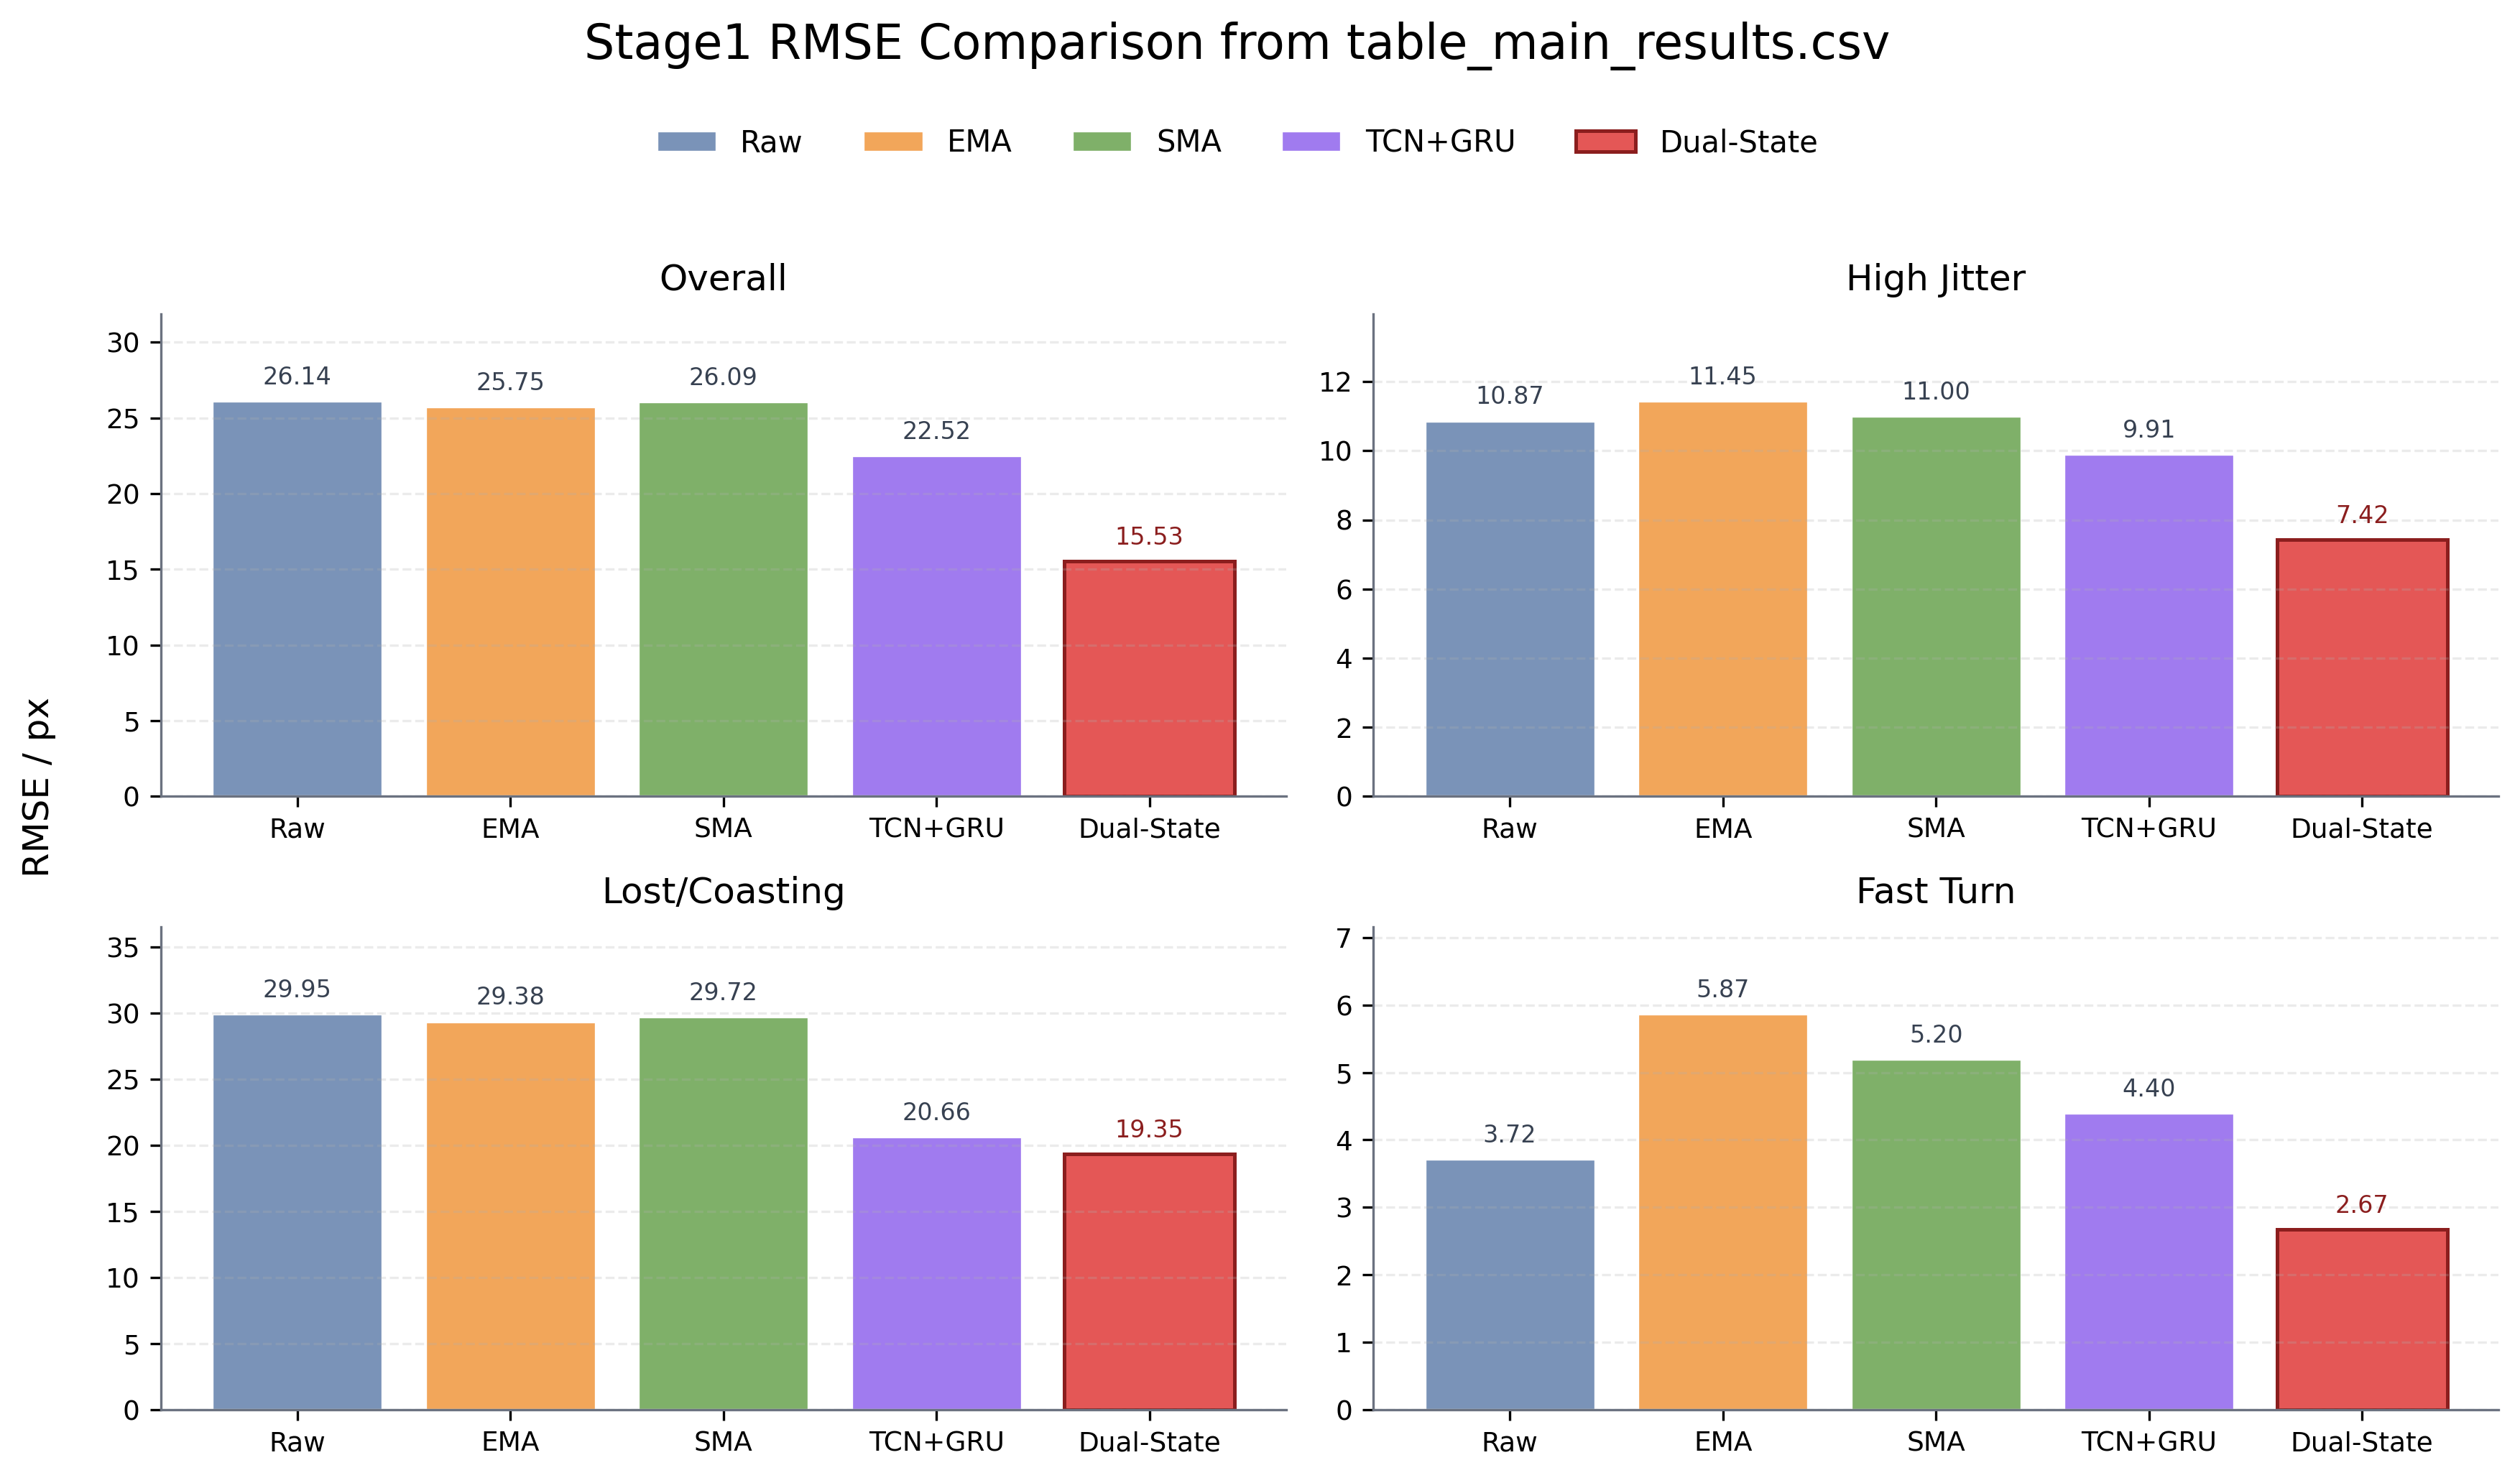
\includegraphics[width=\linewidth]{fig_rmse_comparison.png}
  \caption{不同方法在四个关键口径上的 RMSE 对比。}
  \label{fig:rmse}
\end{figure}

\subsection{显式门控的作用}
Dual-State 的优势并非来自更大的模型规模，而是来自可解释的门控切换。根据正式测试结果，switch gate 的 overall mean 为 0.0565，active ratio 为 0.73\%；在 normal 段，active ratio 为 0；在 high\_jitter 与 fast\_turn 段，active ratio 分别上升到 2.92\% 与 1.46\%。这说明显式门控没有塌缩为常开，也没有在稳态场景中引入不必要的切换。

\begin{figure}[H]
  \centering
  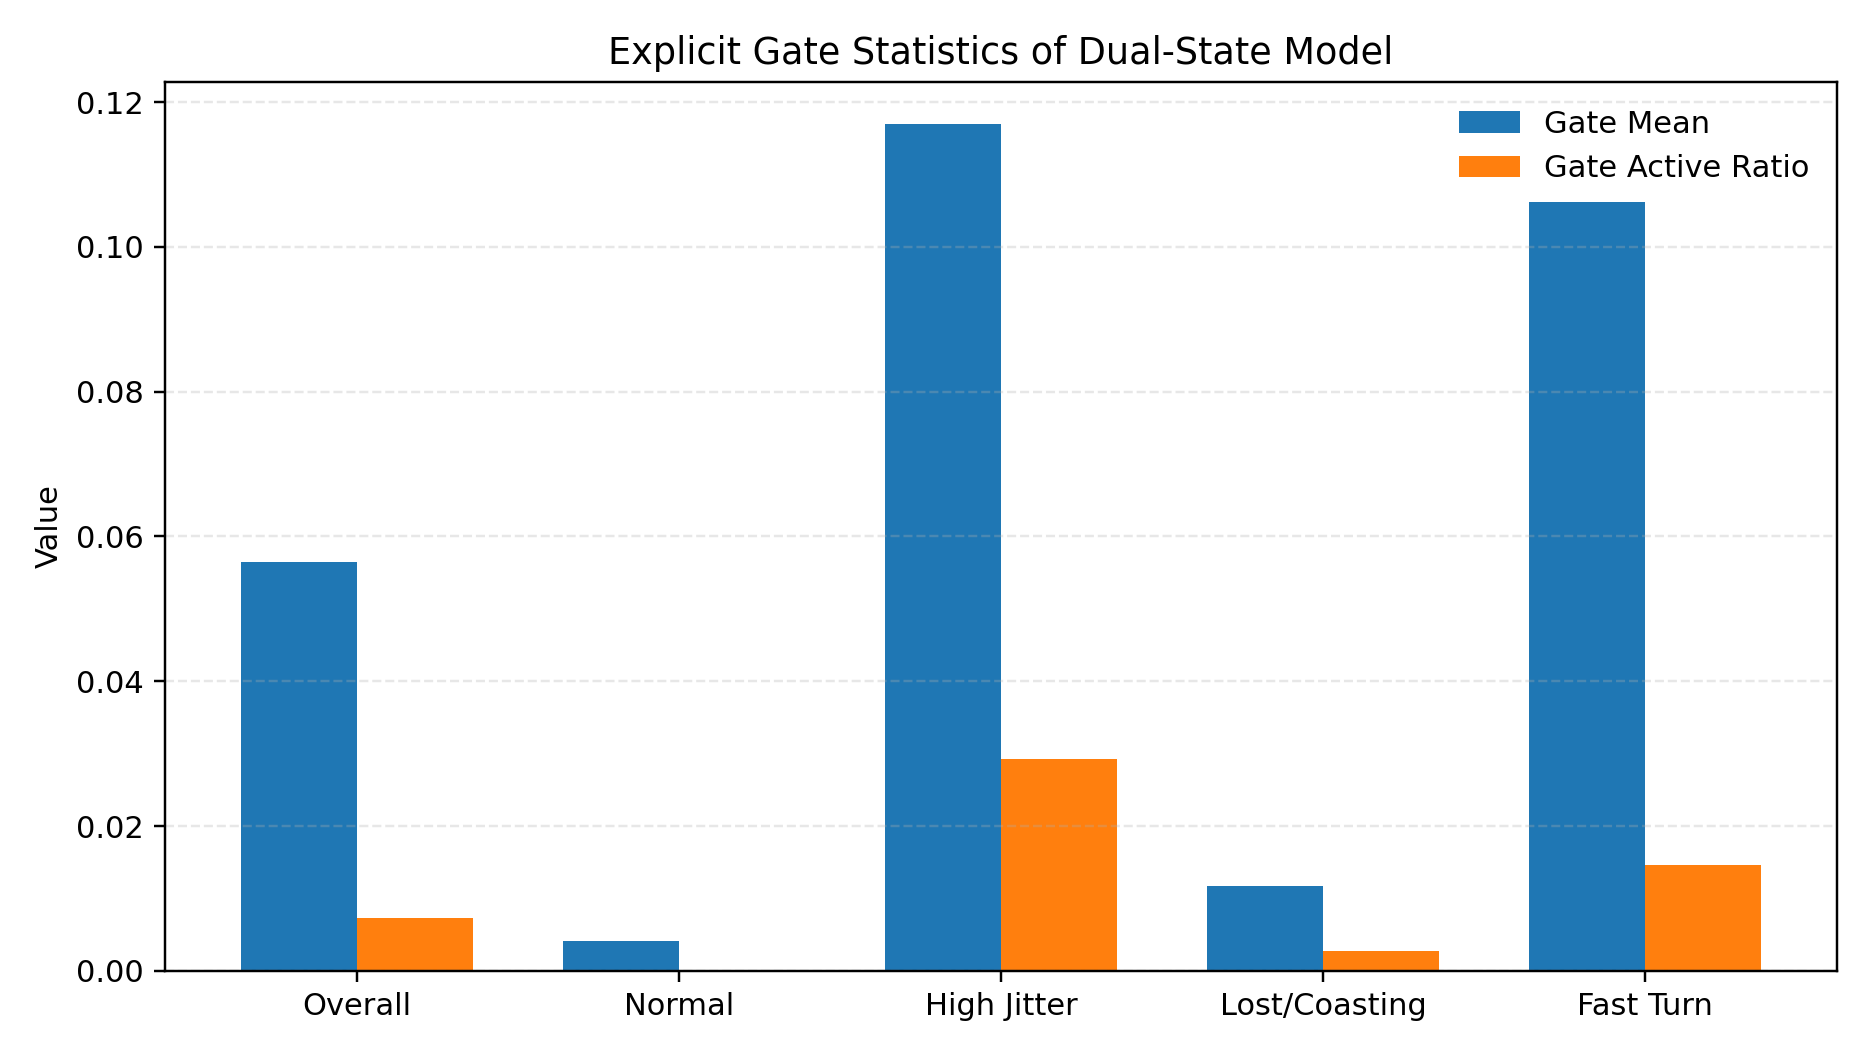
\includegraphics[width=0.82\linewidth]{fig_gate_statistics.png}
  \caption{Dual-State 显式门控在不同场景下的统计特性。}
  \label{fig:gate}
\end{figure}

\subsection{多随机种子稳定性}
图 \ref{fig:seed} 给出了五个随机种子下的复验结果。Dual-State 的 overall RMSE 均值为 25.5369\,px，最好结果为 25.5164\,px，最差结果为 25.5480\,px，波动仅约 0.03\,px，说明当前最优配置并非偶然最优，而是稳定成立。

\begin{table}[H]
  \centering
  \caption{Dual-State 五个随机种子的复验汇总}
  \label{tab:seed}
  \resizebox{\linewidth}{!}{%
  \begin{tabular}{cccccc}
    \toprule
    Seed & Overall RMSE & Overall MAE & High-Jitter RMSE & Lost-Coasting RMSE & Fast-Turn RMSE \\
    \midrule
    41 & 25.5164 & 13.5769 & 9.2768 & 39.3532 & 3.4669 \\
    42 & 25.5425 & 13.6297 & 9.5539 & 39.3532 & 3.8307 \\
    43 & 25.5480 & 13.7945 & 9.5821 & 39.3532 & 3.8994 \\
    44 & 25.5309 & 13.6840 & 9.4197 & 39.3532 & 3.6723 \\
    45 & 25.5467 & 13.6559 & 9.5989 & 39.3532 & 3.8845 \\
    \bottomrule
  \end{tabular}
  }
\end{table}

\begin{figure}[H]
  \centering
  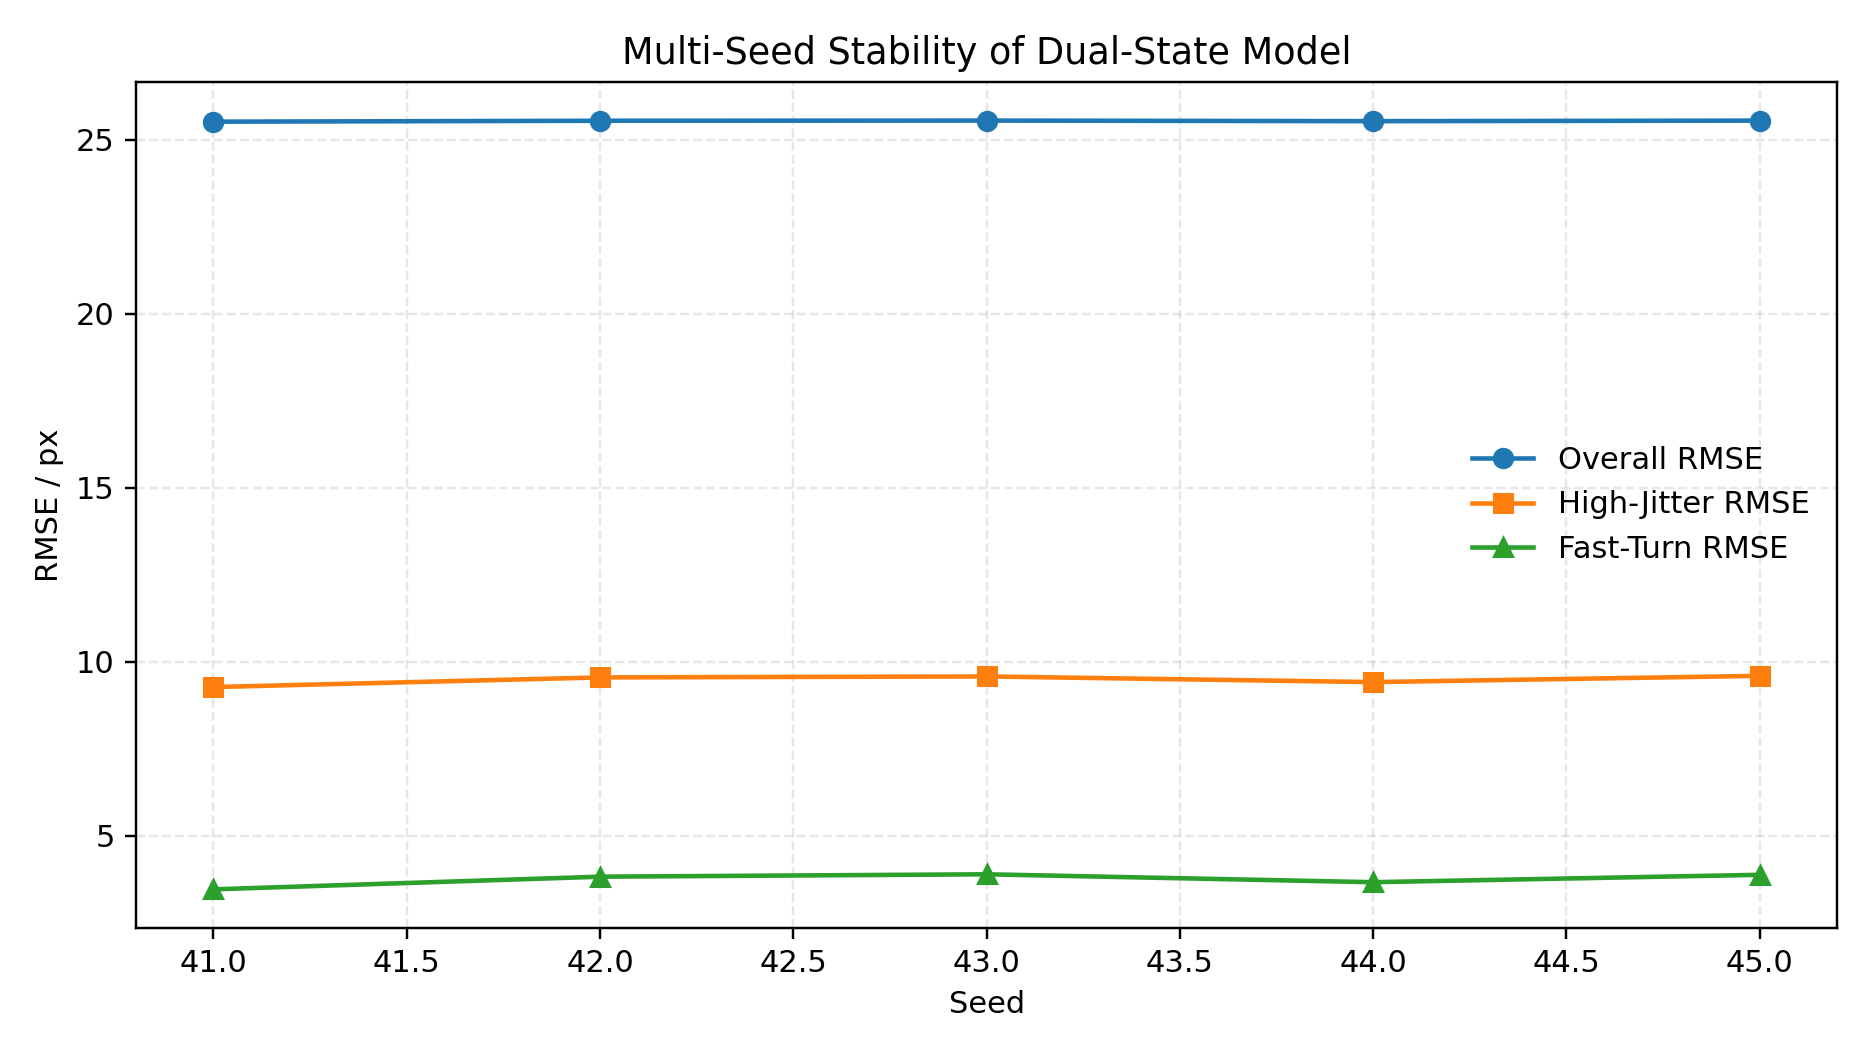
\includegraphics[width=0.82\linewidth]{fig_seed_stability.png}
  \caption{Dual-State 多随机种子稳定性。}
  \label{fig:seed}
\end{figure}

\subsection{典型时序片段分析}
图 \ref{fig:cases} 展示了 stable、jitter、recover 和 turn 四类代表性片段。可以看到，Dual-State 在 jitter 段能明显优于简单平滑方法，减少峰值压扁；在 recover 段保持了比 Raw 更低的波动，同时避免了过强的恢复延迟；在 turn 段，其快速转折性能已经超过 EMA 与 SMA，并略优于 Raw。

\begin{figure}[H]
  \centering
  \begin{subfigure}[b]{0.48\linewidth}
    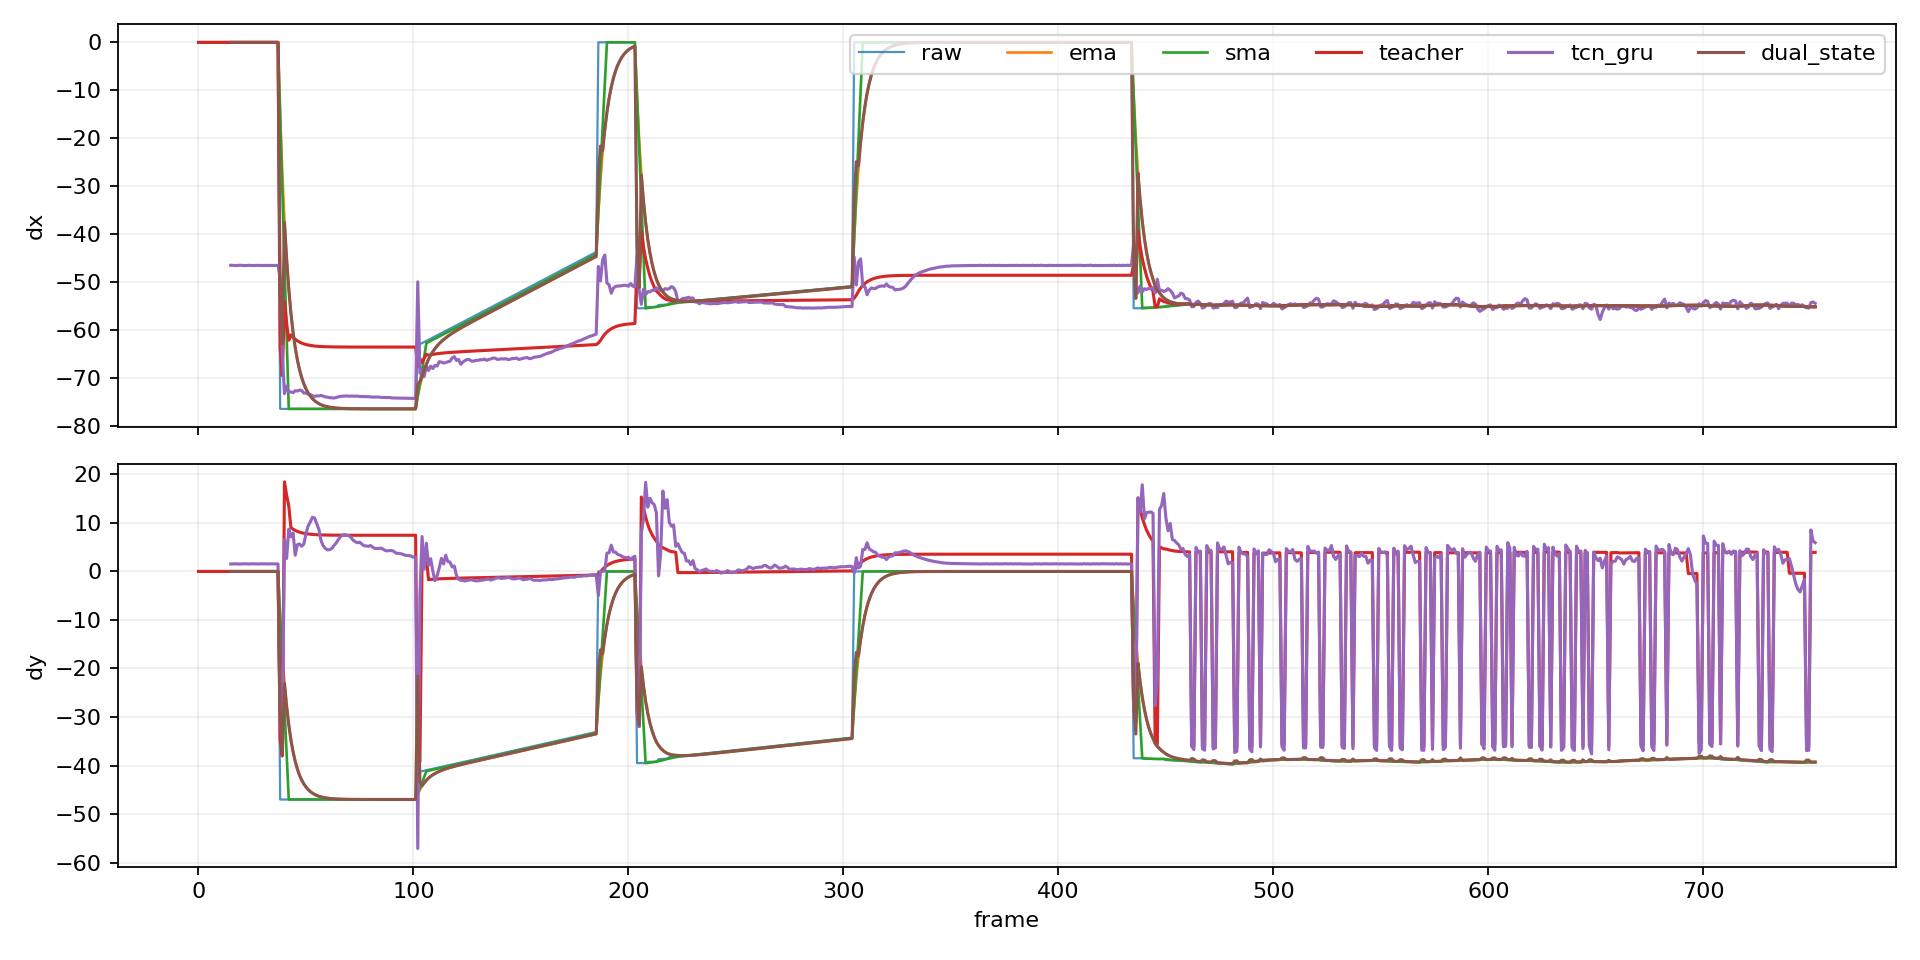
\includegraphics[width=\linewidth]{stable_case.png}
    \caption{Stable}
  \end{subfigure}
  \hfill
  \begin{subfigure}[b]{0.48\linewidth}
    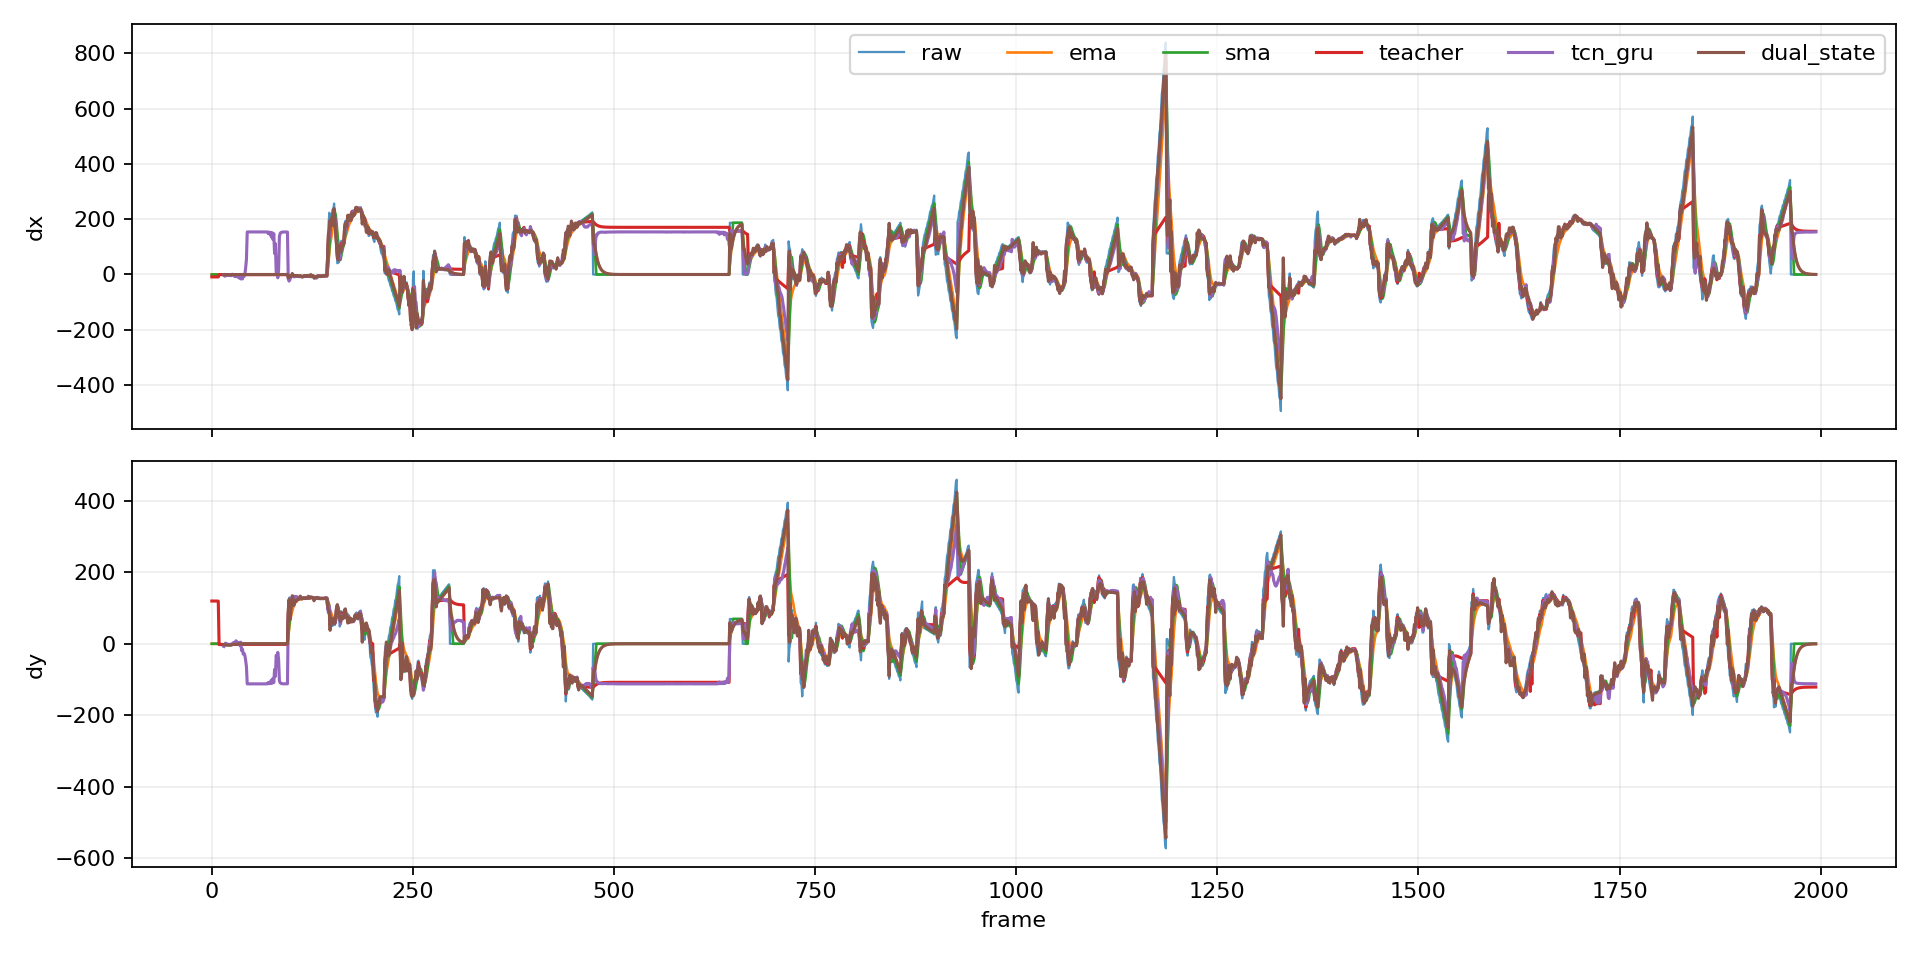
\includegraphics[width=\linewidth]{jitter_case.png}
    \caption{Jitter}
  \end{subfigure}

  \vspace{0.4em}

  \begin{subfigure}[b]{0.48\linewidth}
    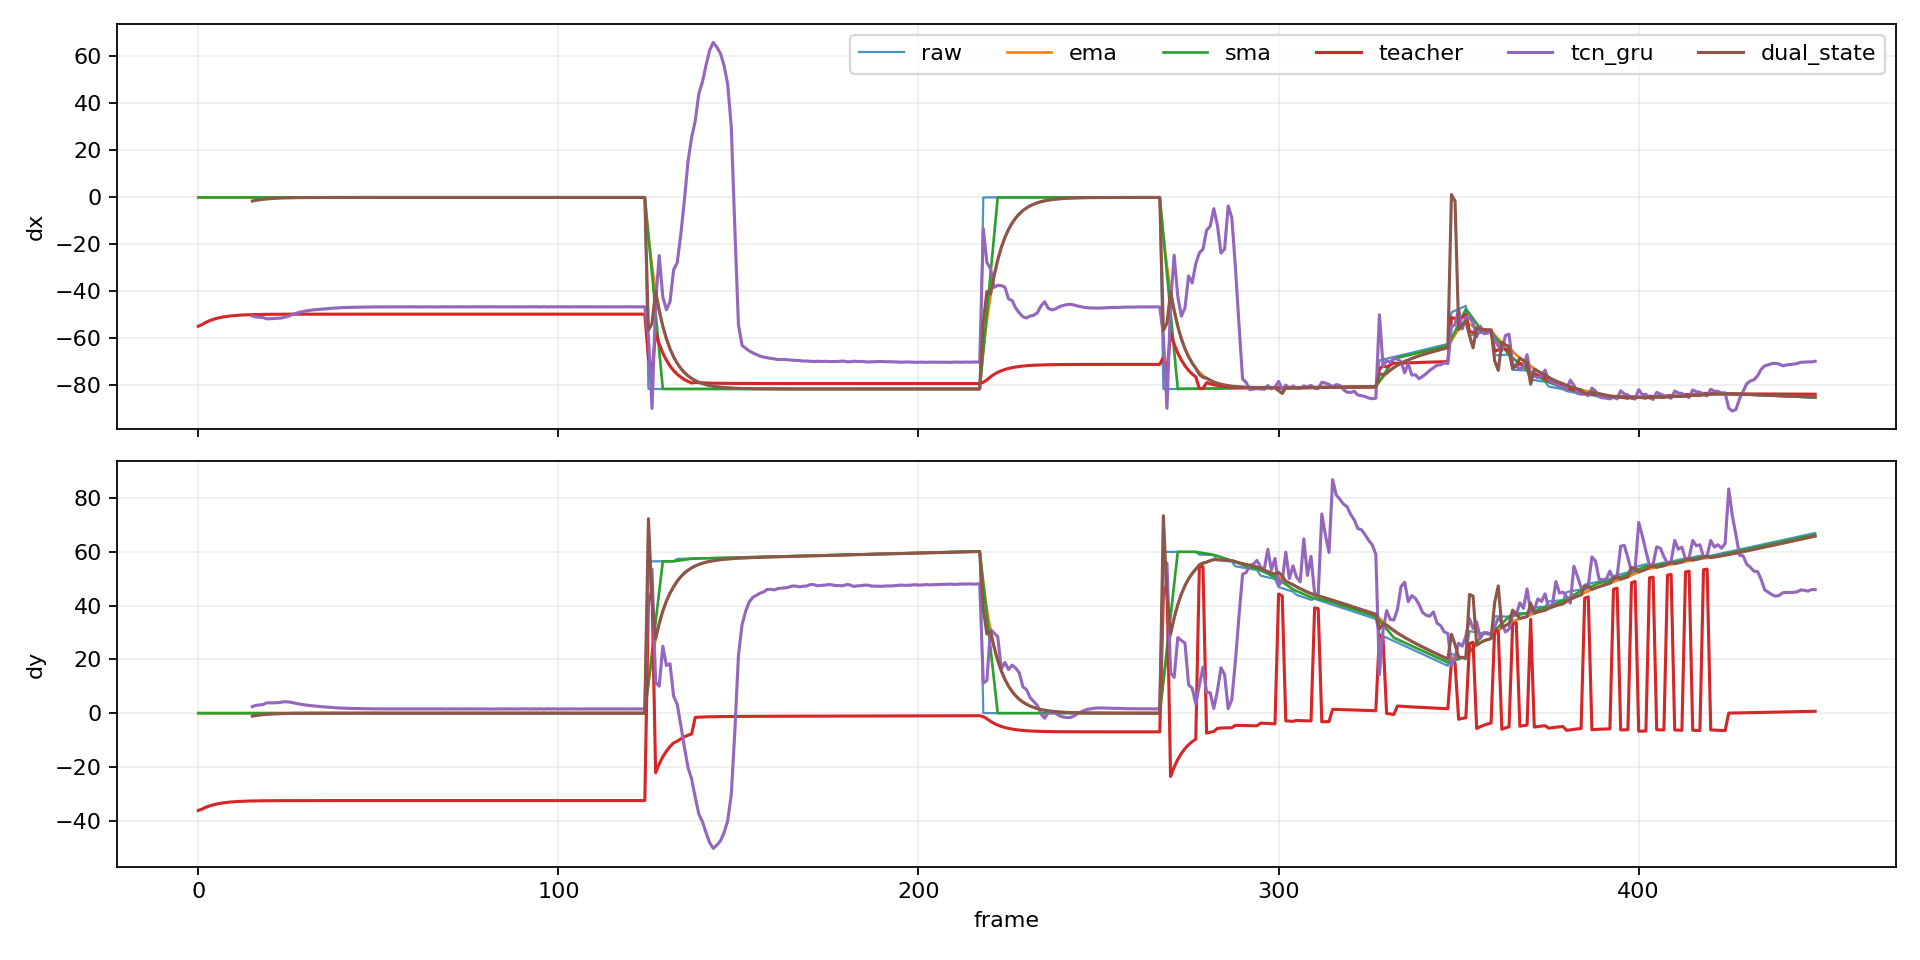
\includegraphics[width=\linewidth]{recover_case.png}
    \caption{Recover}
  \end{subfigure}
  \hfill
  \begin{subfigure}[b]{0.48\linewidth}
    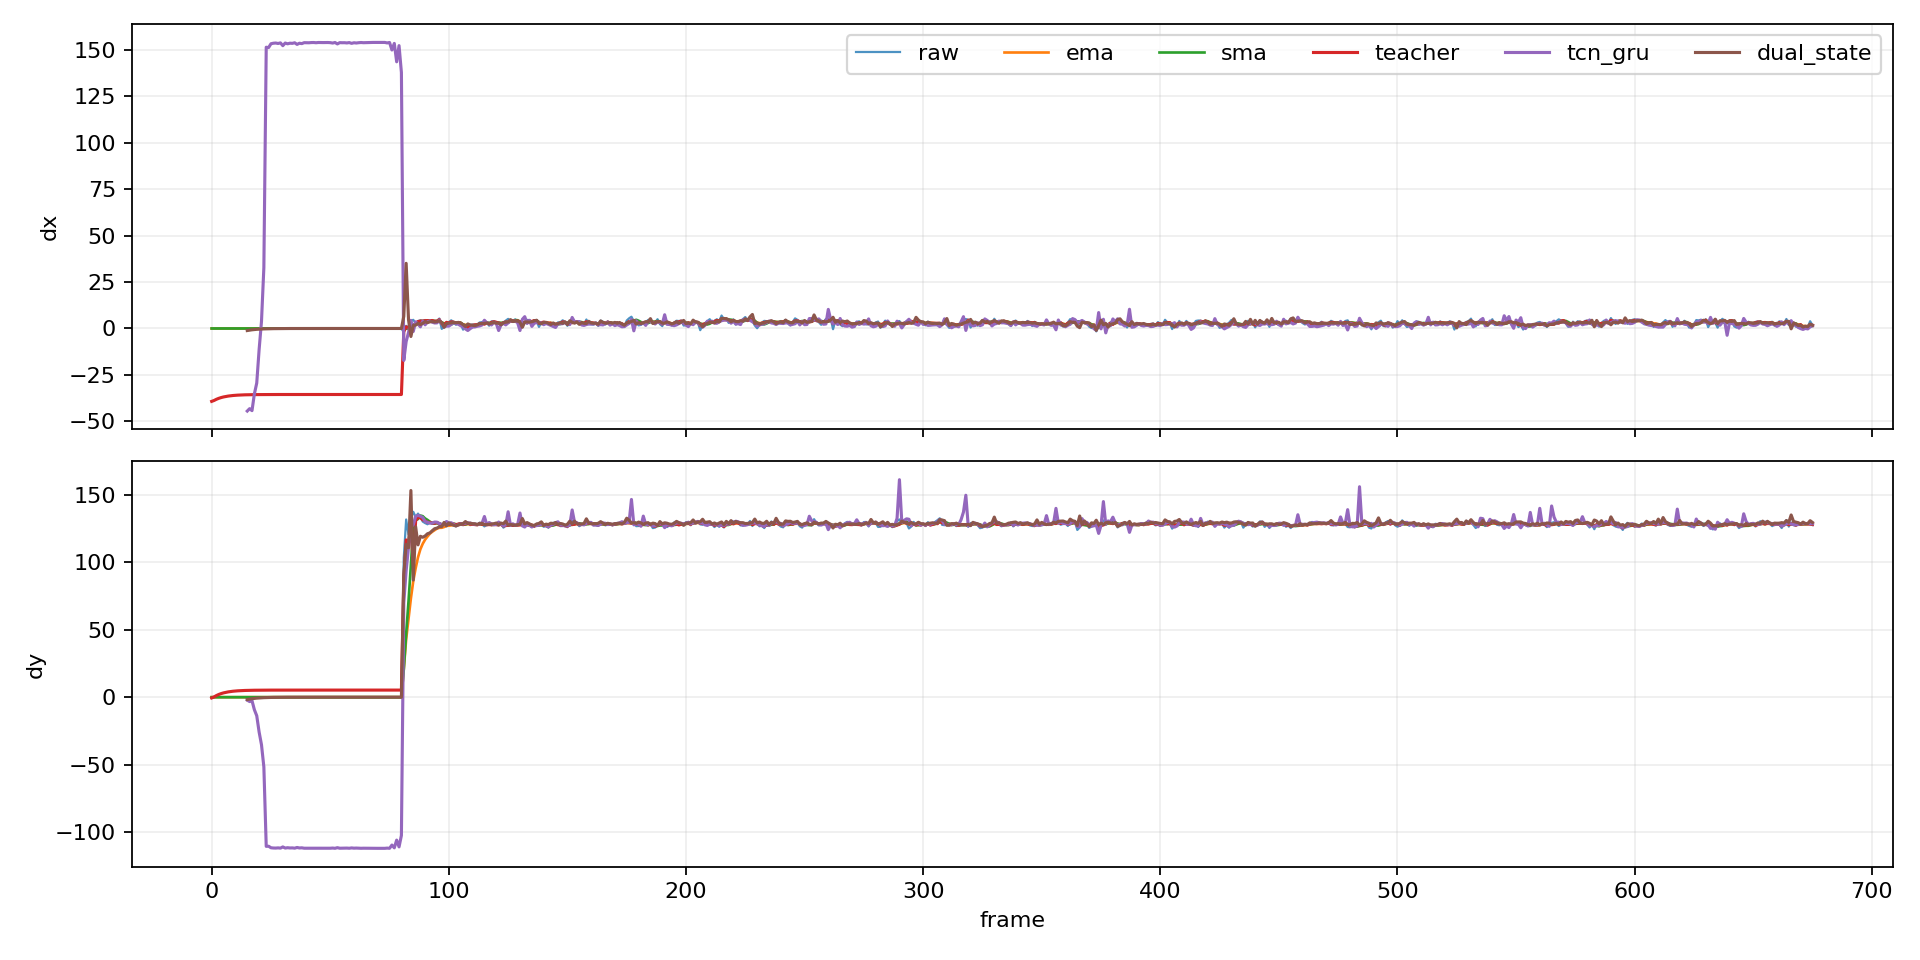
\includegraphics[width=\linewidth]{turn_case.png}
    \caption{Turn}
  \end{subfigure}
  \caption{代表性时序片段中的曲线对比。}
  \label{fig:cases}
\end{figure}

\subsection{在线接入验证}
为了验证方法具有工程可用性，本文将最优 dual-state 模型导出为 ONNX，并接入 C++ 跟踪控制链。回放 smoke 中，模型在第 14 帧开始进入有效推理状态；相机 smoke 中，日志中已可以稳定写出 \texttt{clean\_dx}、\texttt{clean\_dy} 和 \texttt{stage1\_switch\_gate}。这说明该方法不仅离线优于传统基线，而且具备进一步进入 PID 控制链的部署条件。

\section{结论}
本文围绕无人机目标跟踪控制链中的 current clean offset reconstruction 任务，提出了一种显式门控双状态洁净偏差重建方法。与“直接用网络替代滤波器”的思路不同，本文将传统滤波基线、显式门控与事件分支残差修正统一到一条可部署链路中，最终在真实采集数据上同时优于 Raw、EMA 和 SMA 三条传统基线。实验结果表明，所提 dual-state 模型在 overall、high\_jitter、lost\_coasting 和 fast\_turn 四个关键口径上均取得最优结果，并具有较好的随机种子稳定性。后续工作可以在保持当前 clean-only 主版本不退化的前提下，继续探索更高覆盖度的数据采集和与下游控制器的闭环联合优化。

\section*{致谢}
本文稿件中的作者信息、基金信息和单位信息请在正式投稿前补全。

\bibliographystyle{elsarticle-num}
\bibliography{stage1_refs}

\end{document}
